\documentclass[aspectratio=169,10pt]{beamer}

% Compilar con pdfLaTeX
\usepackage[utf8]{inputenc}
\usepackage[T1]{fontenc}
\usepackage[spanish,es-nodecimaldot]{babel}
\usepackage{lmodern}
\usepackage{booktabs}
\usepackage{array}
\usepackage{tikz}
\usetikzlibrary{positioning,arrows.meta,shapes.geometric,fit,calc}
\usepackage{ragged2e}
\usepackage{graphicx}

\usetheme{Madrid}
\usecolortheme{default}

\definecolor{GascoBlue}{RGB}{0,65,105}
\definecolor{GascoCyan}{RGB}{0,145,180}
\definecolor{SoftGray}{RGB}{244,247,250}
\definecolor{GoodGreen}{RGB}{30,130,85}
\definecolor{WarnAmber}{RGB}{154,100,8}
\definecolor{BadRed}{RGB}{161,38,48}

\setbeamercolor{structure}{fg=GascoBlue}
\setbeamercolor{frametitle}{bg=GascoBlue,fg=white}
\setbeamercolor{title}{fg=white,bg=GascoBlue}
\setbeamertemplate{navigation symbols}{}
\setbeamertemplate{footline}[frame number]
\setlength{\parskip}{2pt}

\newcommand{\good}[1]{\textcolor{GoodGreen}{\textbf{#1}}}
\newcommand{\warn}[1]{\textcolor{WarnAmber}{\textbf{#1}}}
\newcommand{\bad}[1]{\textcolor{BadRed}{\textbf{#1}}}
\newcommand{\code}[1]{\texttt{\small #1}}

\title[SVDM -- E3]{Sistema de Venta y Despacho Marino (SVDM)}
\subtitle{Revisión crítica de diseño: construcción, verificación y validación}
\author{Grupo 14}
\institute{Universidad de Concepción}
\date{2026}

\begin{document}

% ============================================================
% 1. Portada
% ============================================================
\begin{frame}[plain]
  \titlepage
  \vfill
  \begin{center}
    \small
    MVP local \textbullet{} 36 pruebas \textbullet{} cobertura 92,38\,\% \textbullet{} 450.083 registros
  \end{center}
\end{frame}

% ============================================================
% 2. Qué cambió desde E2
% ============================================================
\begin{frame}{Qué cambió desde E2}
  % [E3] tiempo objetivo: 25 s
  \begin{columns}[T,onlytextwidth]
    \column{0.32\textwidth}
      \begin{block}{Diseño}
        Construido y ejecutándose en local.\\[1mm]
        RF-1 a RF-10, con roles, persistencia y auditoría.
      \end{block}
    \column{0.32\textwidth}
      \begin{block}{Evidencia}
        36 pruebas y 92,38\,\% de cobertura.\\[1mm]
        8 RNF medidos y dos ciencias con resultados.
      \end{block}
    \column{0.32\textwidth}
      \begin{block}{Validación}
        5 usuarios y protocolo listo.\\[1mm]
        Sesiones planificadas; sin resultados inventados.
      \end{block}
  \end{columns}
  \vspace{2mm}
  \begin{center}
    \large\color{GascoBlue}\textbf{E3 no es una promesa: es el estado verificado del diseño.}
  \end{center}
\end{frame}

% ============================================================
% 3. C1: respuesta a observaciones
% ============================================================
\begin{frame}{C1 · Respuesta a las observaciones de la revisión}
  % [E3] tiempo objetivo: 70 s
  \scriptsize
  \renewcommand{\arraystretch}{1.25}
  \begin{tabular}{@{}p{0.28\textwidth} p{0.38\textwidth} p{0.28\textwidth}@{}}
    \toprule
    \textbf{Observación} & \textbf{Acción adoptada} & \textbf{Evidencia} \\
    \midrule
    Dimensionamiento sin origen & 30 lecturas diarias + 751 horarias por medidor; re-dimensionado a 7.510/mes & RNF-R-2 / R-3 \\
    Modelo incompleto & Modelo del MVP explícito: Cliente, Medidor, Contrato, Lectura, Consolidación; Embarcación/Viaje se difieren y se declaran & SRS \S6.1 / esquema \\
    Alternativas no comparables & Rangos para ALT-1/ALT-3; ALT-2 declarada sin cotización & E2 / pendiente E4 \\
    Riesgos sin disparador & Registro con disparador, probabilidad/impacto y riesgo legal & E1 \S13 \\
    PoC sin magnitud & 30 casos + total; 0 discrepancias & RNF-E-1 \\
    \bottomrule
  \end{tabular}
  \vspace{1.5mm}

  {\tiny Fuente: observaciones de E1 y registro de la revisión anterior.}
\end{frame}

% ============================================================
% 4. C1: iteración 1, datos
% ============================================================
\begin{frame}{C1 · Iteración 1: el dato corrigió el dimensionamiento}
  % [E3] tiempo objetivo: 50 s
  \begin{columns}[T,onlytextwidth]
    \column{0.46\textwidth}
      \begin{block}{Supuesto de E1}
        10 medidores $\times$ 1 lectura/min\\
        $\approx$ 432.000 lecturas/mes\\
        $\approx$ 5,2 millones/año
      \end{block}
    \column{0.50\textwidth}
      \begin{block}{Dato observado}
        30 diarias + 751 horarias por medidor\\
        10 medidores = 7.510/mes\\
        5 años = 450.083 filas
      \end{block}
  \end{columns}
  \vspace{2mm}
  \begin{block}{Decisión y efecto verificado}
    Se re-dimensionaron RNF-R-1 y RNF-R-3. La consolidación con 450.083 filas tiene
    p95 de \good{5,77 ms} y la base ocupa 71,1 MB.
  \end{block}
  \vspace{1mm}
  {\scriptsize Disparador: el dato real no sostenía el supuesto de una lectura por minuto.}
\end{frame}

% ============================================================
% 5. C1: iteración 2, índice
% ============================================================
\begin{frame}{C1 · Iteración 2: el plan de consulta cambió el código}
  % [E3] tiempo objetivo: 50 s
  \begin{columns}[T,onlytextwidth]
    \column{0.48\textwidth}
      \begin{block}{Antes: \code{LIKE}}
        \code{ts LIKE '2026-05\%'}\\[1mm]
        Plan: \code{SEARCH ... (meter\_id=?)}\\[1mm]
        p95 \warn{4,21 ms}
      \end{block}
    \column{0.48\textwidth}
      \begin{block}{Después: rango explícito}
        \code{ts >= ? AND ts < ?}\\[1mm]
        Plan: \code{SEARCH ... (meter\_id=? AND ts>? AND ts<?)}\\[1mm]
        p95 \good{0,20 ms}
      \end{block}
  \end{columns}
  \vspace{2mm}
  \begin{block}{Efecto verificado}
    RNF-R-1 con 5 años: p95 de \warn{46,97 ms} a \good{5,77 ms}.\\
    El cambio se aplicó en \code{getReadings} y en las consultas del resumen.
  \end{block}
\end{frame}

% ============================================================
% 6. C2: estado de la construcción
% ============================================================
\begin{frame}{C2 · Estado de la construcción}
  % [E3] tiempo objetivo: 50 s
  \begin{columns}[T,onlytextwidth]
    \column{0.48\textwidth}
      \begin{block}{MVP local}
        \begin{tikzpicture}[
          node distance=4mm,
          box/.style={draw=GascoBlue, rounded corners, fill=SoftGray, align=center,
                      font=\scriptsize, minimum height=7mm, text width=2.4cm},
          arr/.style={-{Latex}, thick, GascoBlue}
        ]
          \node[box] (ui) {Navegador\\UI};
          \node[box, below=of ui] (api) {API\\Node HTTP};
          \node[box, below=of api] (db) {SQLite\\SVDM};
          \node[box, right=of api, text width=2.0cm] (ad) {Adaptadores\\eGauge\\WiseData\\EIA / SAP};
          \draw[arr] (ui) -- (api);
          \draw[arr] (api) -- (db);
          \draw[arr, dashed] (ad) -- (api);
        \end{tikzpicture}
      \end{block}
    \column{0.50\textwidth}
      \begin{block}{Requisitos}
      \scriptsize
      \begin{tabular}{@{}ll@{}}
        \toprule
        \textbf{Requisito} & \textbf{Estado} \\
        \midrule
        RF-1 a RF-6 (Must) & \good{Implementadas} \\
        RF-7 a RF-10 (Should) & \good{Implementadas} \\
        RF-11 (Could) & \warn{Pendiente} \\
        RF-12 (Won't) & \warn{Excluida} \\
        \bottomrule
      \end{tabular}
      \vspace{1mm}

      {\tiny RF-1/RF-3 usan datos de la planilla, sin WiseData real; RF-2 usa fixture; RF-6 es auth local; RF-7 es simulador; RF-11 está pendiente.}
      \end{block}
  \end{columns}
  \vspace{1mm}
  \begin{block}{Repositorio y calidad}
    7 commits \textbullet{} CI en GitHub Actions \textbullet{} 36 pruebas \textbullet{} cobertura 92,38\,\%
  \end{block}
\end{frame}

% ============================================================
% 7. C2: demo
% ============================================================
\begin{frame}{C2 · Demostración en vivo}
  % [E3] tiempo objetivo: 120 s
  \begin{columns}[T,onlytextwidth]
    \column{0.44\textwidth}
      \begin{enumerate}
        \item Analista ve la alerta del Cliente B.
        \item Abre la alerta, revisa la medición y corrige el valor con motivo.
        \item Genera la consolidación.
        \item La envía a revisión.
        \item Aprobador aprueba; queda bloqueada.
        \item Auditoría registra cada acción.
      \end{enumerate}
      \vspace{1mm}
      {\scriptsize Datos en SQLite. Sin video ni maqueta.\\
      Si falla la red, se usa la base sembrada y las capturas de respaldo.}
    \column{0.54\textwidth}
      \begin{block}{Estados y control}
        \centering
        \begin{tikzpicture}[
          node distance=4mm,
          state/.style={draw, rounded corners, align=center, font=\scriptsize,
                        minimum height=7mm, text width=3.4cm},
          arr/.style={-{Latex}, thick, GascoBlue}
        ]
          \node[state, fill=red!8, draw=BadRed] (a) {Alerta abierta};
          \node[state, below=of a, fill=orange!10, draw=WarnAmber] (b) {Corrección\\con motivo};
          \node[state, below=of b, fill=blue!8, draw=GascoBlue] (c) {En revisión};
          \node[state, below=of c, fill=green!10, draw=GoodGreen] (d) {Aprobada e inmutable};
          \draw[arr] (a) -- (b);
          \draw[arr] (b) -- (c);
          \draw[arr] (c) -- (d);
        \end{tikzpicture}
        \vspace{1mm}

        {\tiny Auditoría: actor, rol, fecha, acción y motivo.}
      \end{block}
      {\scriptsize Capturas de la interfaz en las láminas de respaldo.}
  \end{columns}
\end{frame}

% ============================================================
% 8. C3: complejidad
% ============================================================
\begin{frame}{C3 · Ciencias (1/2): complejidad e índices}
  % [E3] tiempo objetivo: 50 s
  \begin{columns}[T,onlytextwidth]
    \column{0.50\textwidth}
      \begin{block}{Modelo}
        Índice B-tree \code{(meter\_id, ts)}.\\
        Costo esperado: $O(\log N + k)$, con $k$ lecturas del período.
      \end{block}
    \column{0.46\textwidth}
      \centering
      \scriptsize
      \begin{tabular}{@{}lrr@{}}
        \toprule
        Consulta & p95 & Filas \\
        \midrule
        \code{LIKE} & 4,21 ms & 30 \\
        Rango & \good{0,20 ms} & 30 \\
        \bottomrule
      \end{tabular}
  \end{columns}
  \vspace{2mm}
  \begin{block}{Resultado}
    450.000 filas y 71,1 MB. La consolidación completa (RNF-R-1) queda en
    \good{5,77 ms} de p95 con 5 años de datos.
  \end{block}
  {\scriptsize Medición directa sobre SQLite, 30 corridas por consulta.}
\end{frame}

% ============================================================
% 9. C3: anomalías
% ============================================================
\begin{frame}{C3 · Ciencias (2/2): anomalías con datos reales}
  % [E3] tiempo objetivo: 50 s
  \begin{columns}[T,onlytextwidth]
    \column{0.52\textwidth}
      \begin{block}{Regla de Tukey}
        $IQR = Q3 - Q1$\\
        Límites: $Q1 - 1{,}5\,IQR$ y $Q3 + 1{,}5\,IQR$
      \end{block}
      \begin{itemize}
        \item 30 lecturas diarias: \warn{1 candidato} (479,12 kWh).
        \item 751 horarias: \warn{12 caídas}, \warn{13 saltos}, 667 ceros.
        \item 11 de 12 caídas seguidas de salto: reinicio del acumulador.
      \end{itemize}
    \column{0.44\textwidth}
      \begin{block}{Inyección controlada}
        6 anomalías conocidas\\[1mm]
        \begin{tabular}{@{}ll@{}}
          VP & 6 \\
          FP & 0--1 \\
          FN & 0 \\
          Recall & \good{100\,\%} \\
        \end{tabular}
      \end{block}
  \end{columns}
  \vspace{1mm}
  \begin{block}{Decisión}
    Dos reglas (caída negativa + Tukey) y confirmación humana.
    La alerta es un disparador de revisión, no un veredicto automático.
  \end{block}
\end{frame}

% ============================================================
% 10. C4: verificación y RNF
% ============================================================
\begin{frame}{C4 · Verificación y medición de RNF}
  % [E3] tiempo objetivo: 70 s
  \scriptsize
  \renewcommand{\arraystretch}{1.2}
  \begin{tabular}{@{}llll@{}}
    \toprule
    \textbf{RNF} & \textbf{Objetivo} & \textbf{Valor obtenido} & \textbf{Veredicto} \\
    \midrule
    R-1 Consolidación & $\leq$ 5 min & 5,77 ms con 450.083 filas & \good{Cumple} \\
    R-2 Ingesta & $\leq$ 60 s & 10,9 ms de mediana & \good{Cumple} \\
    R-3 Volumen 5 años & sin degradar R-1 & 450.083 filas, 71,1 MB & \good{Cumple} \\
    E-1 Exactitud & 0 disc., $\leq$ 1 CLP & 0 líneas; 0,0044 CLP & \good{Cumple} \\
    E-2 Integridad & 0 duplicados & 0 antes y después & \good{Cumple} \\
    S-2 RBAC & mínimo privilegio & 8/8 controles & \good{Cumple} \\
    S-4 Auditoría & 100\,\% eventos & 4/4 acciones & \good{Cumple} \\
    M-1 Cobertura & 70 / 90\,\% & 92,38 / 92,38\,\% & \good{Cumple} \\
    \bottomrule
  \end{tabular}
  \vspace{1.5mm}

  {\tiny 36 pruebas. Parciales o pendientes: D-1, D-2, D-3, S-1, S-3, U-1, U-2, M-2 (ver \code{docs/rnf.md}).}
  \vspace{1mm}

  \begin{block}{Lectura}
    Los RNF críticos cumplen con margen. Los pendientes dependen de infraestructura o de usuarios y se declaran como tales.
  \end{block}
\end{frame}

% ============================================================
% 11. C5: validación
% ============================================================
\begin{frame}{C5 · Validación con usuarios}
  % [E3] tiempo objetivo: 40 s
  % [COMPLETAR] Reemplazar el bloque "Estado" por la tabla de resultados
  % cuando estén las 5 sesiones y se ejecute npm run validate:analyze.
  \begin{columns}[T,onlytextwidth]
    \column{0.52\textwidth}
      \begin{block}{Diseño}
        5 participantes del perfil analista/aprobador.\\
        Tarea principal de punta a punta.\\
        Umbral: \textbf{4 de 5 sin ayuda} (RNF-U-2).
      \end{block}
      \begin{itemize}
        \item Se miden éxito, tiempo, ayuda, errores, facilidad y confianza.
        \item Instrumento, consentimiento y registro listos.
        \item Análisis reproducible con \code{npm run validate:analyze}.
      \end{itemize}
    \column{0.44\textwidth}
      \begin{block}{Estado}
        Sesiones planificadas.\\[1mm]
        Los resultados se reportan en \code{docs/validacion/resultados.md}.
      \end{block}
      \begin{block}{Compromiso}
        No se reportan resultados hasta completar las 5 sesiones.
      \end{block}
  \end{columns}
\end{frame}

% ============================================================
% 12. C6: costos, riesgos y replanificación
% ============================================================
\begin{frame}{C6 · Costos, riesgos y replanificación}
  % [E3] tiempo objetivo: 40 s
  \scriptsize
  \begin{tabular}{@{}lll@{}}
    \toprule
    \textbf{Ítem} & \textbf{Estimado} & \textbf{Ejecutado} \\
    \midrule
    Infraestructura & 200--800 USD/año & \good{0 USD} (local) \\
    Herramientas & 0 USD & 0 USD \\
    Horas de equipo & 1.080 h & \warn{registro en curso} \\
    \bottomrule
  \end{tabular}
  \vspace{1.5mm}
  \begin{columns}[T,onlytextwidth]
    \column{0.48\textwidth}
      \begin{block}{Riesgos materializados}
        Sin Azure ni credenciales $\rightarrow$ adaptadores locales.\\
        Granularidad distinta $\rightarrow$ re-dimensionado.\\
        Alcance $\rightarrow$ RF-12 excluida.
      \end{block}
    \column{0.48\textwidth}
      \begin{block}{Replanificación}
        Comprometemos validación, E4 y E5.\\
        Excluimos Azure, SAP/Entra reales y RF-12.
      \end{block}
  \end{columns}
  \vspace{1mm}
  \begin{block}{Lectura}
    El costo de infraestructura ejecutado es 0 porque el MVP corre local; el estimado corresponde a Azure.
    El registro de horas se completa con la bitácora del equipo.
  \end{block}
\end{frame}

% ============================================================
% 13. Cierre
% ============================================================
\begin{frame}{Cierre}
  % [E3] tiempo objetivo: 15 s
  \begin{block}{Construido y medido}
    RF-1 a RF-10 \textbullet{} 36 pruebas \textbullet{} RNF críticos medidos \textbullet{} 2 ciencias con resultados.
  \end{block}
  \begin{block}{Comprometido}
    Resultados de validación \textbullet{} informe E4 \textbullet{} defensa E5.
  \end{block}
  \begin{block}{Fuera de alcance}
    Azure \textbullet{} SAP/Entra reales \textbullet{} RF-12.
  \end{block}
  \vfill
  \centering
  {\Large\color{GascoBlue}\textbf{Gracias · Preguntas}}
\end{frame}

% ============================================================
% Respaldo
% ============================================================
\appendix

\begin{frame}{Respaldo · Requisitos funcionales}
  \scriptsize
  \begin{tabular}{@{}lll@{}}
    \toprule
    \textbf{RF} & \textbf{Descripción} & \textbf{Estado} \\
    \midrule
    RF-1 & Ingesta de lecturas & Implementado \\
    RF-2 & Precio EIA & Implementado (fixture) \\
    RF-3 & Cálculo de consumo & Implementado \\
    RF-4 & Consolidación & Implementado \\
    RF-5 & Revisión y aprobación & Implementado \\
    RF-6 & Acceso por rol & Implementado (local) \\
    RF-7 & Envío a SAP & Simulado \\
    RF-8 & Alertas & Implementado \\
    RF-9 & Corrección de lectura & Implementado \\
    RF-10 & Auditoría & Implementado \\
    RF-11 & Exportación & Pendiente \\
    RF-12 & Gastos marítimos y portal & Excluido \\
    \bottomrule
  \end{tabular}
\end{frame}

\begin{frame}{Respaldo · RNF medidos y pendientes}
  \scriptsize
  \begin{columns}[T,onlytextwidth]
    \column{0.50\textwidth}
      \textbf{Medidos}
      \begin{itemize}
        \item R-1: 5,77 ms (450k filas)
        \item R-2: 10,9 ms
        \item R-3: 450.083 filas, 71,1 MB
        \item E-1: 0 líneas fuera de tolerancia
        \item E-2: 0 duplicados
        \item S-2: 8/8; S-4: 4/4
        \item M-1: 92,38 / 92,38 \%
      \end{itemize}
    \column{0.46\textwidth}
      \textbf{Parciales o pendientes}
      \begin{itemize}
        \item D-1: disponibilidad mensual
        \item D-2: RPO/RTO
        \item D-3: falla de fuente
        \item S-1: Entra ID + MFA
        \item S-3: TLS/cifrado
        \item U-1: WCAG
        \item U-2: validación
        \item M-2: lint/observabilidad
      \end{itemize}
  \end{columns}
\end{frame}

\begin{frame}{Respaldo · Arquitectura}
  \centering
  \begin{tikzpicture}[
    node distance=5mm,
    box/.style={draw=GascoBlue, rounded corners, fill=SoftGray, align=center,
                font=\scriptsize, minimum height=8mm, text width=2.6cm},
    ext/.style={draw=GascoCyan, dashed, rounded corners, fill=white, align=center,
                font=\scriptsize, minimum height=7mm, text width=2.2cm},
    arr/.style={-{Latex}, thick, GascoBlue}
  ]
    \node[box] (ui) {Navegador\\Resumen / Consolidación / Clientes};
    \node[box, below=of ui] (api) {API Node HTTP\\roles, estados, auditoría};
    \node[box, below=of api] (db) {SQLite\\lecturas, consolidaciones, líneas};
    \node[ext, right=of api] (eg) {eGauge / WiseData\\adaptador};
    \node[ext, above=of eg] (eia) {EIA\\precio};
    \node[ext, below=of eg] (sap) {SAP\\simulador};
    \draw[arr] (ui) -- (api);
    \draw[arr] (api) -- (db);
    \draw[arr, dashed] (eg) -- (api);
    \draw[arr, dashed] (eia) -- (api);
    \draw[arr, dashed] (sap) -- (api);
  \end{tikzpicture}
  \vspace{2mm}
  {\scriptsize El diseño mantiene puertos y adaptadores: los simuladores se reemplazan por los sistemas reales sin cambiar el dominio.}
\end{frame}

\begin{frame}{Respaldo · Validación: tareas}
  \scriptsize
  \begin{enumerate}
    \item \textbf{T1 (principal):} entrar como analista, resolver la alerta del Cliente B con una lectura manual, generar la consolidación, enviarla a revisión, entrar como aprobador y aprobar.
    \item \textbf{T2:} encontrar el evento de ingreso manual en Auditoría.
    \item \textbf{T3:} explicar la trazabilidad de una línea: kWh $\times$ precio $\times$ tipo de cambio; kWh $\times$ factor.
    \item \textbf{T4 (opcional):} rechazar con motivo una consolidación preparada.
  \end{enumerate}
  \vspace{1mm}
  {\scriptsize Métricas: éxito, tiempo, nivel de ayuda (0/1/2), errores, facilidad y confianza (1--7).}
\end{frame}

\begin{frame}{Respaldo · Repositorio y reproducibilidad}
  \small
  \begin{itemize}
    \item \textbf{Repositorio:} \code{github.com/Vicente-021/proyectoInf}
    \item \textbf{Arranque:} \code{npm run seed} y \code{npm start}
    \item \textbf{Pruebas:} \code{npm test} (33) y \code{npm run coverage}
    \item \textbf{Evidencia:} \code{npm run measure}, \code{npm run sciences}, \code{npm run validate:analyze}
    \item \textbf{Sin dependencias npm:} Node 24, \code{node:sqlite}, \code{node:http}, \code{node:test}.
  \end{itemize}
  \vspace{1mm}
  {\scriptsize El repositorio incluye CI para pruebas y cobertura.}
\end{frame}

\begin{frame}{Respaldo · Riesgos vigentes}
  \scriptsize
  \begin{tabular}{@{}p{0.30\textwidth} p{0.36\textwidth} p{0.28\textwidth}@{}}
    \toprule
    \textbf{Riesgo} & \textbf{Mitigación} & \textbf{Disparador} \\
    \midrule
    Credenciales/APIs no disponibles & Adaptadores y simuladores; carga por archivo & Semana sin acceso \\
    Granularidad distinta a la esperada & Re-dimensionar y validar con datos reales & Lecturas fuera de rango \\
    Cambio de contrato/factor & Factor por contrato y auditoría & Nueva versión de contrato \\
    Baja adopción & Validación con usuarios y capacitación & Tarea no completada \\
    Datos personales & Minimización, RBAC y auditoría & Acceso indebido \\
    \bottomrule
  \end{tabular}
\end{frame}

\begin{frame}{Respaldo · captura de consolidación}
  \centering
  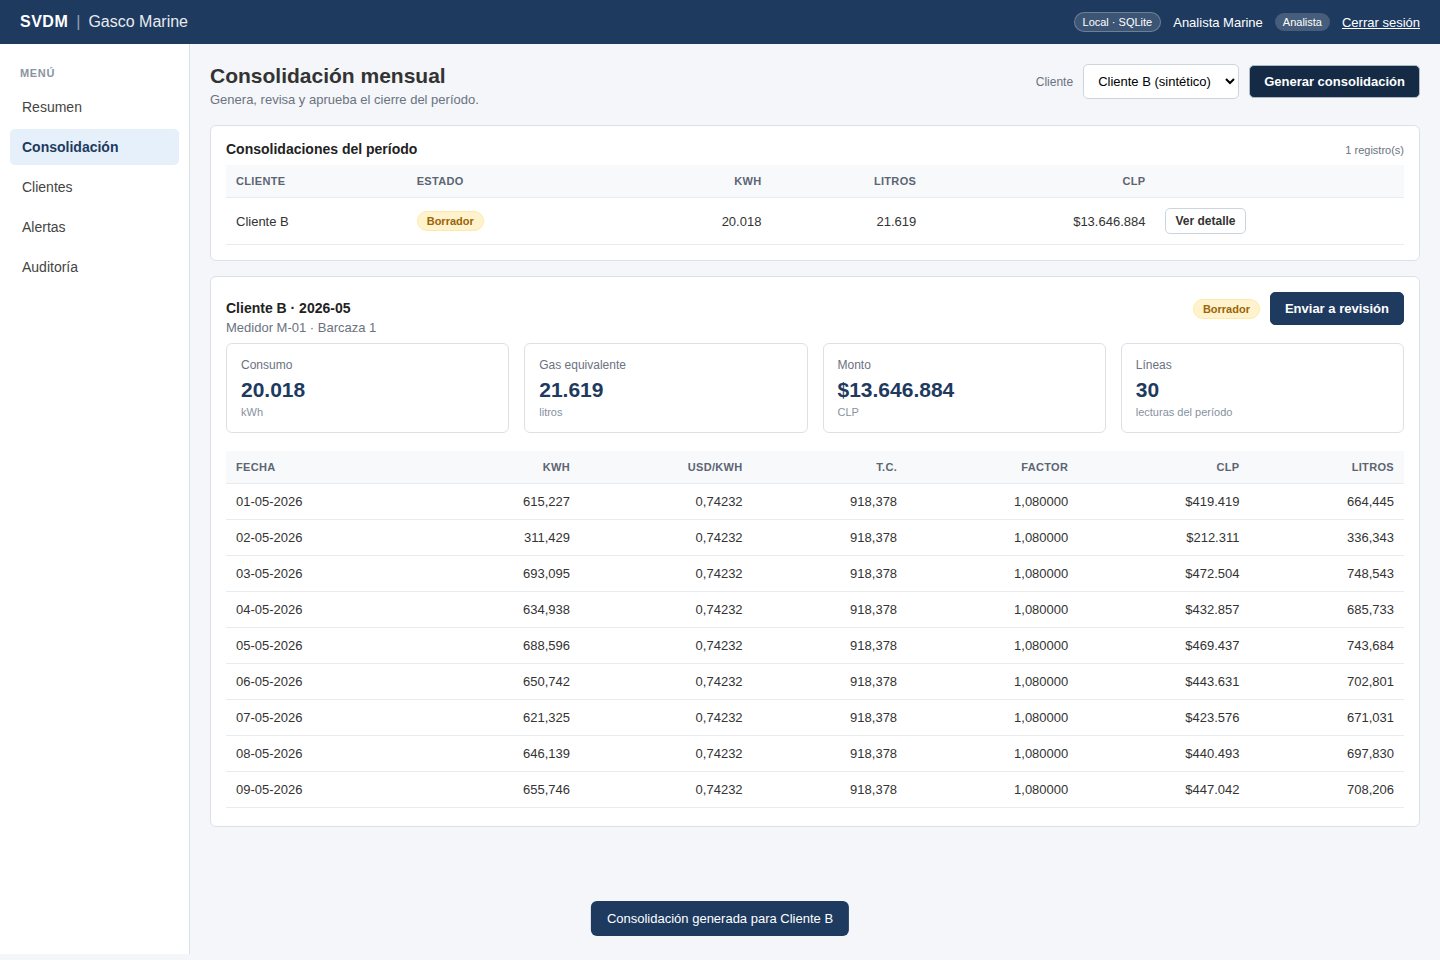
\includegraphics[width=\textwidth,height=0.72\textheight,keepaspectratio]{img/consolidacion.png}
  \vspace{1mm}

  {\scriptsize Captura de la interfaz: consolidación generada, con totales, líneas y acciones de revisión.}
\end{frame}

\begin{frame}{Respaldo · resumen y consolidación aprobada}
  \begin{columns}[T,onlytextwidth]
    \column{0.48\textwidth}
      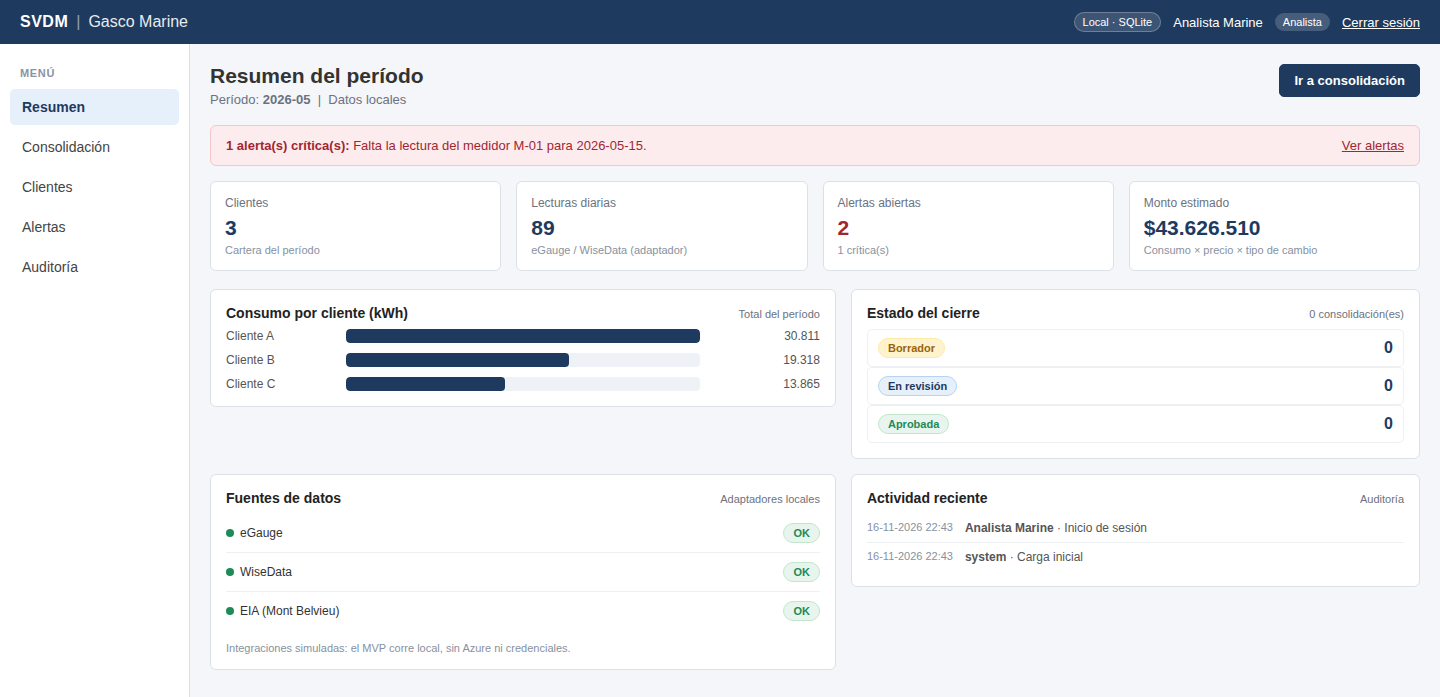
\includegraphics[width=\linewidth]{img/resumen.png}
    \column{0.48\textwidth}
      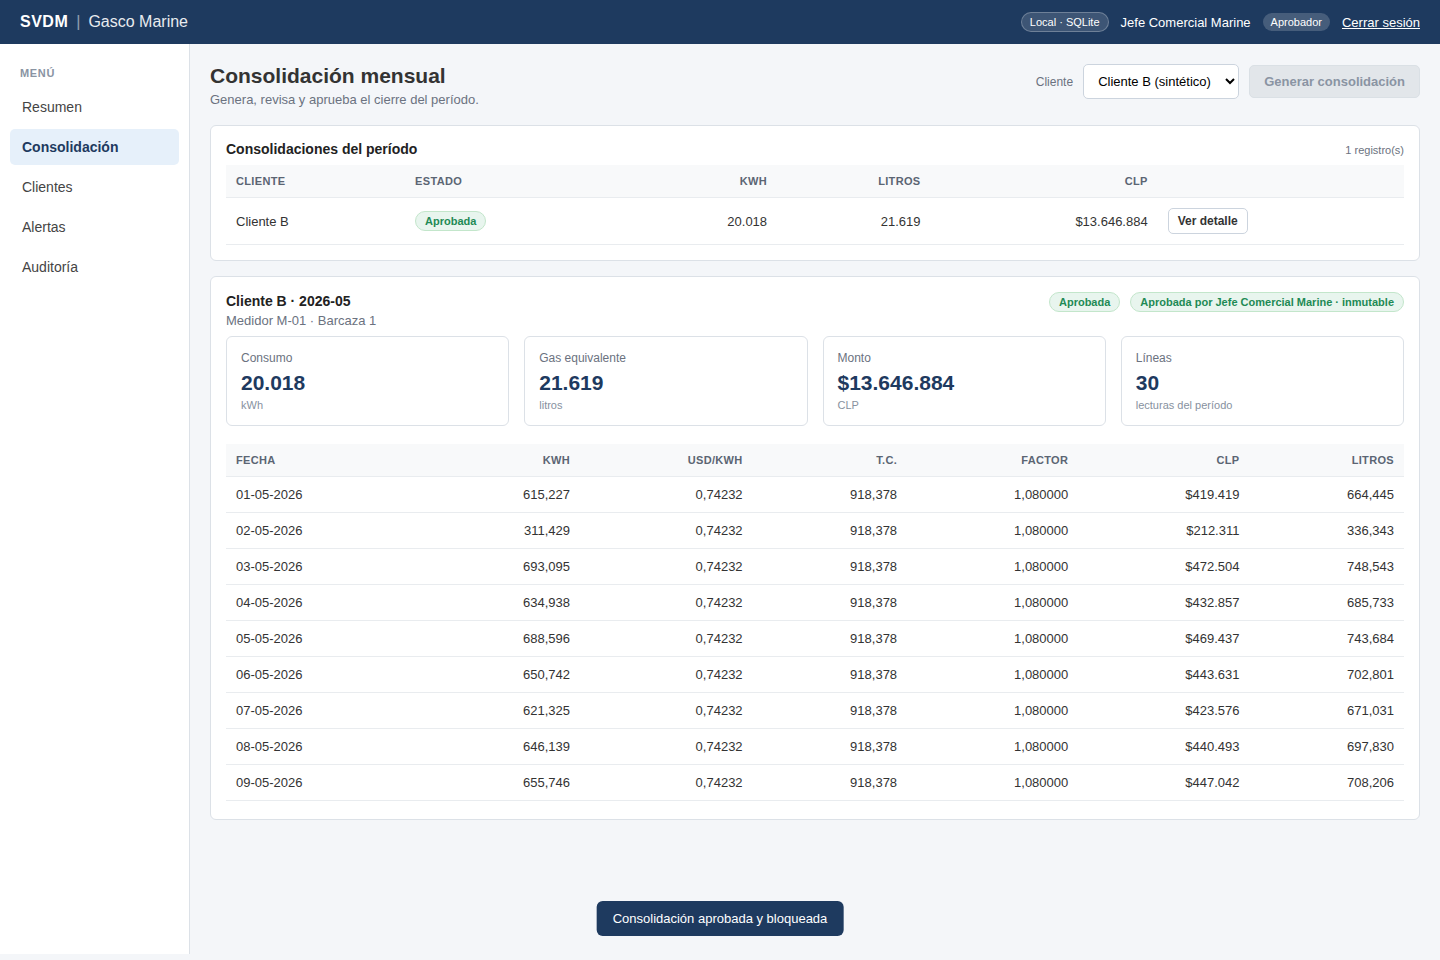
\includegraphics[width=\linewidth]{img/aprobada.png}
  \end{columns}
  \vspace{1mm}

  {\scriptsize Izquierda: tablero de resumen. Derecha: consolidación aprobada e inmutable.}
\end{frame}

\end{document}
